This section is going to touch upon various technical aspects of the setup that is used to develop and test the application. In particular, the set-up which is used for the reproduction of attacks is going to be described and references to tools and other extensions that were employed to analyze the attacks are going to be given.
Initially, three virtual machines were used to reproduce the attacks and to test various aspects of the application. This is depicted in \autoref{fig:tech-set-up}. This set-up has been used to integrate ARP-spoofing and network-scanning capabilities. The local network-scanning is an integral part of the application. Since the objective is to develop an easy-to-use tool, we do not want to bother the user to find out who or what is connected to the local network. The user should be able to simply `plug-and-play' in whatever environment the application is used. This is a feature similar to the list of capabilities of tools such as \href{https://github.com/Ettercap/ettercap}{\textit{Ettercap} (a suite for man-in-the-middle attacks) } and \href{https://github.com/nmap/nmap}{\textit{Nmap} (network mapper)}. Once ARP-spoofing and local-network scans were correctly implemented and assessed to be employable in different network settings (e.g. by changing network interfaces by exploiting \texttt{ifconfig} commands: \texttt{ifconfig iface down/up}), the set-up was extended with other functionalities for different testing purposes. 

\begin{figure}[t!]
	\centering
	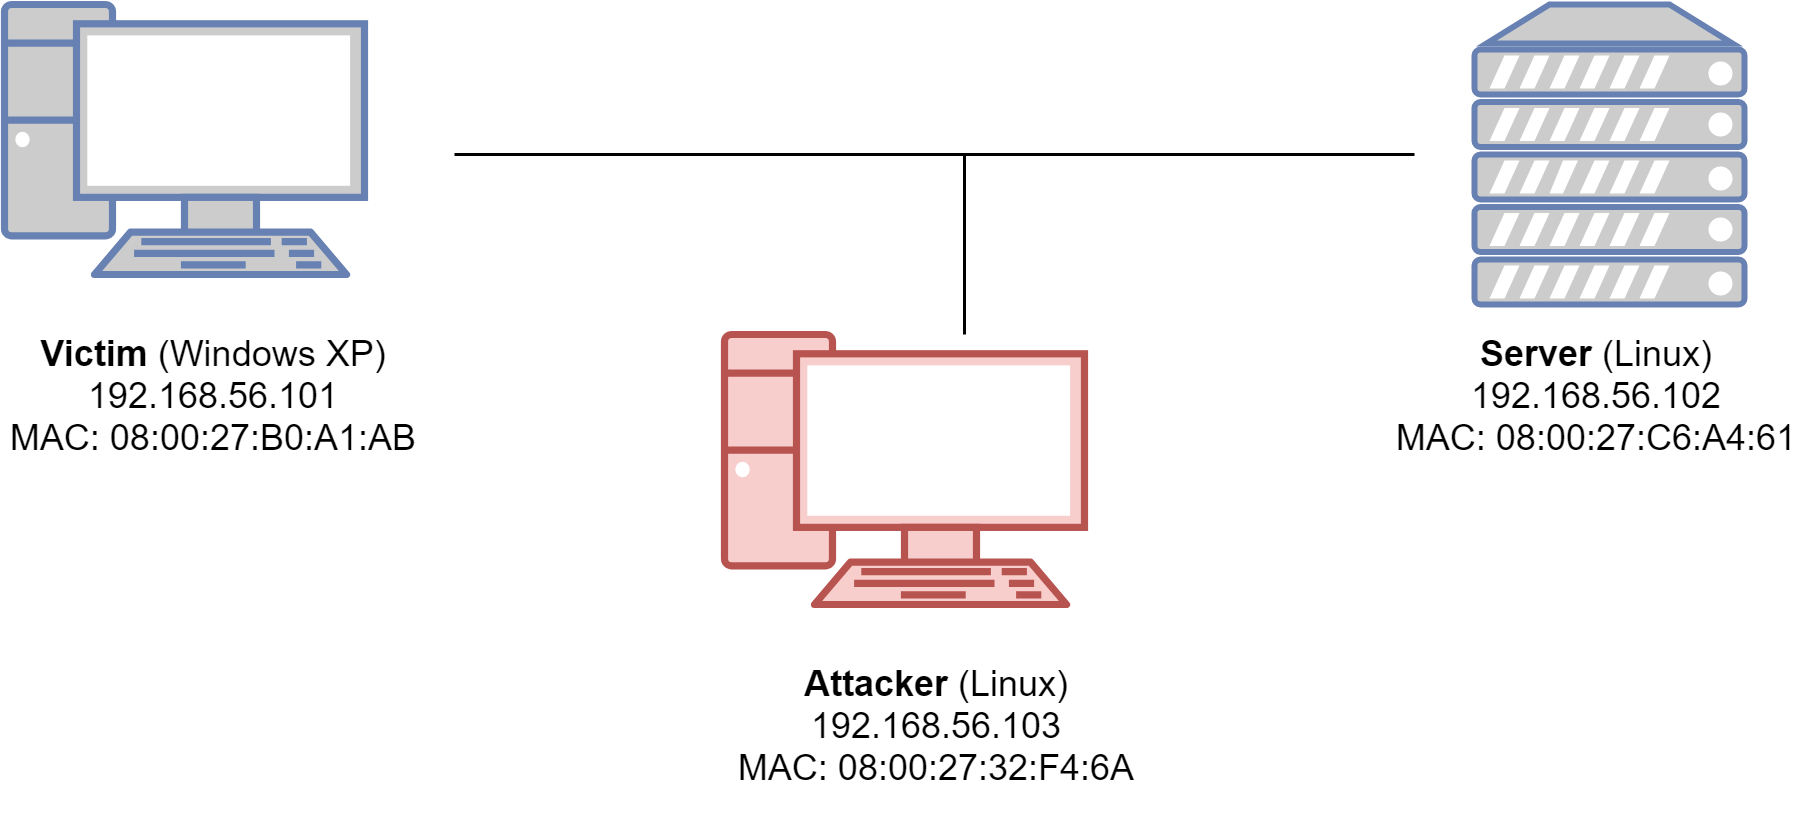
\includegraphics[width=0.4\textwidth]{img/tech_set_up.png}
	\caption{
		Set-up which is employed for application-development \& attack-reproduction and -analysis }
	\label{fig:tech-set-up}
\end{figure}

For starters, a simple web-page was hosted on the Linux server depicted on the right in \autoref{fig:tech-set-up}. This web-page has been developed to test various aspects of the applications such as the filtering of \texttt{HTTP} requests, Cookies et cetera. The dummy page is depicted in \autoref{fig:dummy_page}. One can simply set and retrieve payloads according to the tests on would like to employ.\\

\begin{figure}[h!]
	\centering
	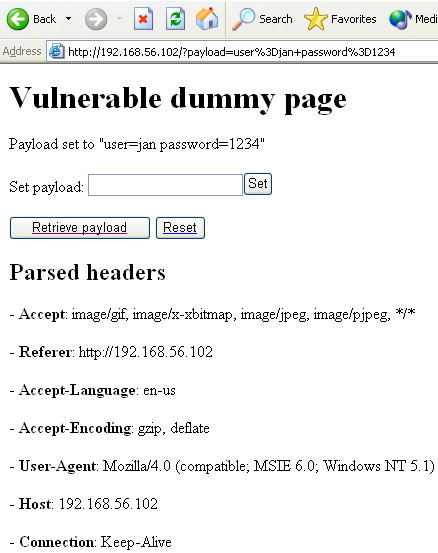
\includegraphics[width=0.5\textwidth]{img/dummy_page.png}
	\caption{
		The dummy page that was hosted on the server for testing purposes}
	\label{fig:dummy_page}
\end{figure}

Once these tests were conducted and were deemed to be successful, a fourth entity was added to the set-up depicted in \autoref{fig:dummy_page}. In particular, a second server (a copy of the first server) was added to the environment to assess the injection capabilities (e.g. \texttt{IMG-}tag injection). The victim sets a cookie in communications with this new (second) server. Subsequently, the cookie can be retrieved through an \texttt{IMG-}tag injection which contains a reference to this second server when traffic is send from the victim to the original server (as is explained in the previous section). \\

Aside from this set-up, \href{https://www.wireshark.org/}{\textit{Wireshark}} (\texttt{version: 2.2.6)} was used both in the initial development and testing phase (e.g. ARP-spoofing, local-network scan) and later phases aimed at packet modifications (e.g. injections etc.). In addition, various scripts/automated tests have been written which eased the development and testing process of the application. These tests can be found under \href{https://github.com/akbokha/fhttp/tree/master/test}{ /test/} and are (primarily) designed for the aforementioned network setting.\\

As explained before, the tool has to be easy-to-use since we both want to reach a large (tech-savvy) audience and want to showcase to less technical people how vulnerable one can be in various everyday settings by demonstrating how quick one can learn the relevant concepts (considering that we have little to no prior experience) and techniques and process them into a fully-fledged application. Hopefully, this will be a warning to them what Cyber-security researchers and engineers (or `hackers') can do when you are their `bullseye'. The afore-stated incentive behind the development of this easy-to-use application goes, therefore, hand-in-hand with the development of a graphical user-interface (GUI). Python's de-facto GUI package \href{https://wiki.python.org/moin/TkInter}{\textit{TkInter}} has, therefore, been used to develop the GUI. This does, however, introduce (yet another) dependency. The applications has been developed in- and tested with \texttt{TkInter 8.5}. In addition, \href{https://github.com/secdev/scapy}{\texttt{Scapy}} was, of course, used. The application has been extensively tested using \texttt{version: 2.3.2}. An update to \texttt{2.4.0} was considered and has been evaluated, but this affected the performance of the local network scanner. 


% [max 700 words]
% - Used tools/dependencies
% - Arp spoofing
% - Network analysis
% - accepted encoding headers
% - img tag injection
% - filtering of cookies